\documentclass{article}

% packages
\usepackage{amsmath, amsthm, thmtools, amsfonts, amssymb, luacode, catchfile, tikzducks, hyperref, ifthen}
\ifcsname c@kobocompile\endcsname
	\usepackage[a5paper, total={1072pt, 1448pt}, margin=10pt, includeheadfoot]{geometry} % set page margins
\else
	\usepackage[a4paper, margin=50pt, includeheadfoot]{geometry}
\fi
\usepackage[shortlabels]{enumitem}
\usepackage[skip=3pt, indent=0pt]{parskip}

% language
\usepackage[bidi=basic, layout=tabular, provide=*]{babel}
\ifcsname c@english\endcsname
	\babelprovide[main, import]{english}
\else
	\babelprovide[main, import]{hebrew}
	\babelprovide{rl}
\fi
%\babelfont{rm}{Libertinus Serif}
\babelfont{rm}[Renderer=Harfbuzz]{Libertinus Serif}
\babelfont{sf}{Libertinus Sans}
\babelfont{tt}{Libertinus Mono}

% style
\AddToHook{cmd/section/before}{\clearpage}	% Add line break before section
\linespread{1.3}
\setcounter{secnumdepth}{0}		% Remove default number tags from sections, this won't do well with theorems
\AtBeginDocument{\setlength{\belowdisplayskip}{3pt}}
\AtBeginDocument{\setlength{\abovedisplayskip}{3pt}}
\graphicspath{ {../images/} }

% operators
\DeclareMathOperator\cis{cis}
\DeclareMathOperator\Sp{Sp}
\DeclareMathOperator\tr{tr}
\DeclareMathOperator\im{Im}
\DeclareMathOperator\re{Re}
\DeclareMathOperator\diag{diag}
\DeclareMathOperator*\lowlim{\underline{lim}}
\DeclareMathOperator*\uplim{\overline{lim}}
\DeclareMathOperator\rng{rng}
\DeclareMathOperator\Sym{Sym}
\DeclareMathOperator\Arg{Arg}
\DeclareMathOperator\Log{Log}
\DeclareMathOperator\dom{dom}
\DeclareMathOperator\supp{Supp}
\DeclareMathOperator\var{Var}
\DeclareMathOperator\cov{Cov}

% commands
%\renewcommand\qedsymbol{\textbf{מש''ל}}
%\renewcommand\qedsymbol{\fbox{\emoji{lizard}}}
\newcommand{\Aa}[0]{\mathcal{A}}
\newcommand{\Bb}[0]{\mathcal{B}}
\newcommand{\CC}[0]{\mathbb{C}}
\newcommand{\Cc}[0]{\mathcal{C}}
\newcommand{\EE}[0]{\mathbb{E}}
\newcommand{\FF}[0]{\mathbb{F}}
\newcommand{\Ff}[0]{\mathcal{F}}
\newcommand{\Ii}[0]{\mathcal{I}}
\newcommand{\Gg}[0]{\mathcal{G}}
\newcommand{\Ll}[0]{\mathcal{L}}
\newcommand{\Mm}[0]{\mathcal{M}}
\newcommand{\NN}[0]{\mathbb{N}}
\newcommand{\Nn}[0]{\mathcal{N}}
\newcommand{\PP}[0]{\mathbb{P}}
\newcommand{\Pp}[0]{\mathcal{P}}
\newcommand{\QQ}[0]{\mathbb{Q}}
\newcommand{\RR}[0]{\mathbb{R}}
\newcommand{\Rr}[0]{\mathcal{R}}
\newcommand{\Ss}[0]{\mathcal{S}}
\newcommand{\TT}[0]{\mathbb{T}}
\newcommand{\Uu}[0]{\mathcal{U}}
\newcommand{\Vv}[0]{\mathcal{V}}
\newcommand{\Ww}[0]{\mathcal{W}}
\newcommand{\ZZ}[0]{\mathbb{Z}}
\newcommand{\acts}[0]{\circlearrowright}
\newcommand{\explain}[2] {
	\begin{flalign*}
		 && \text{#2} && \text{#1}
	\end{flalign*}
}
\newcommand{\maketitleprint}[0]{ \begin{center}
	%\begin{tikzpicture}[scale=3]
	%	\duck[graduate=gray!20!black, tassel=red!70!black]
	%\end{tikzpicture}	
	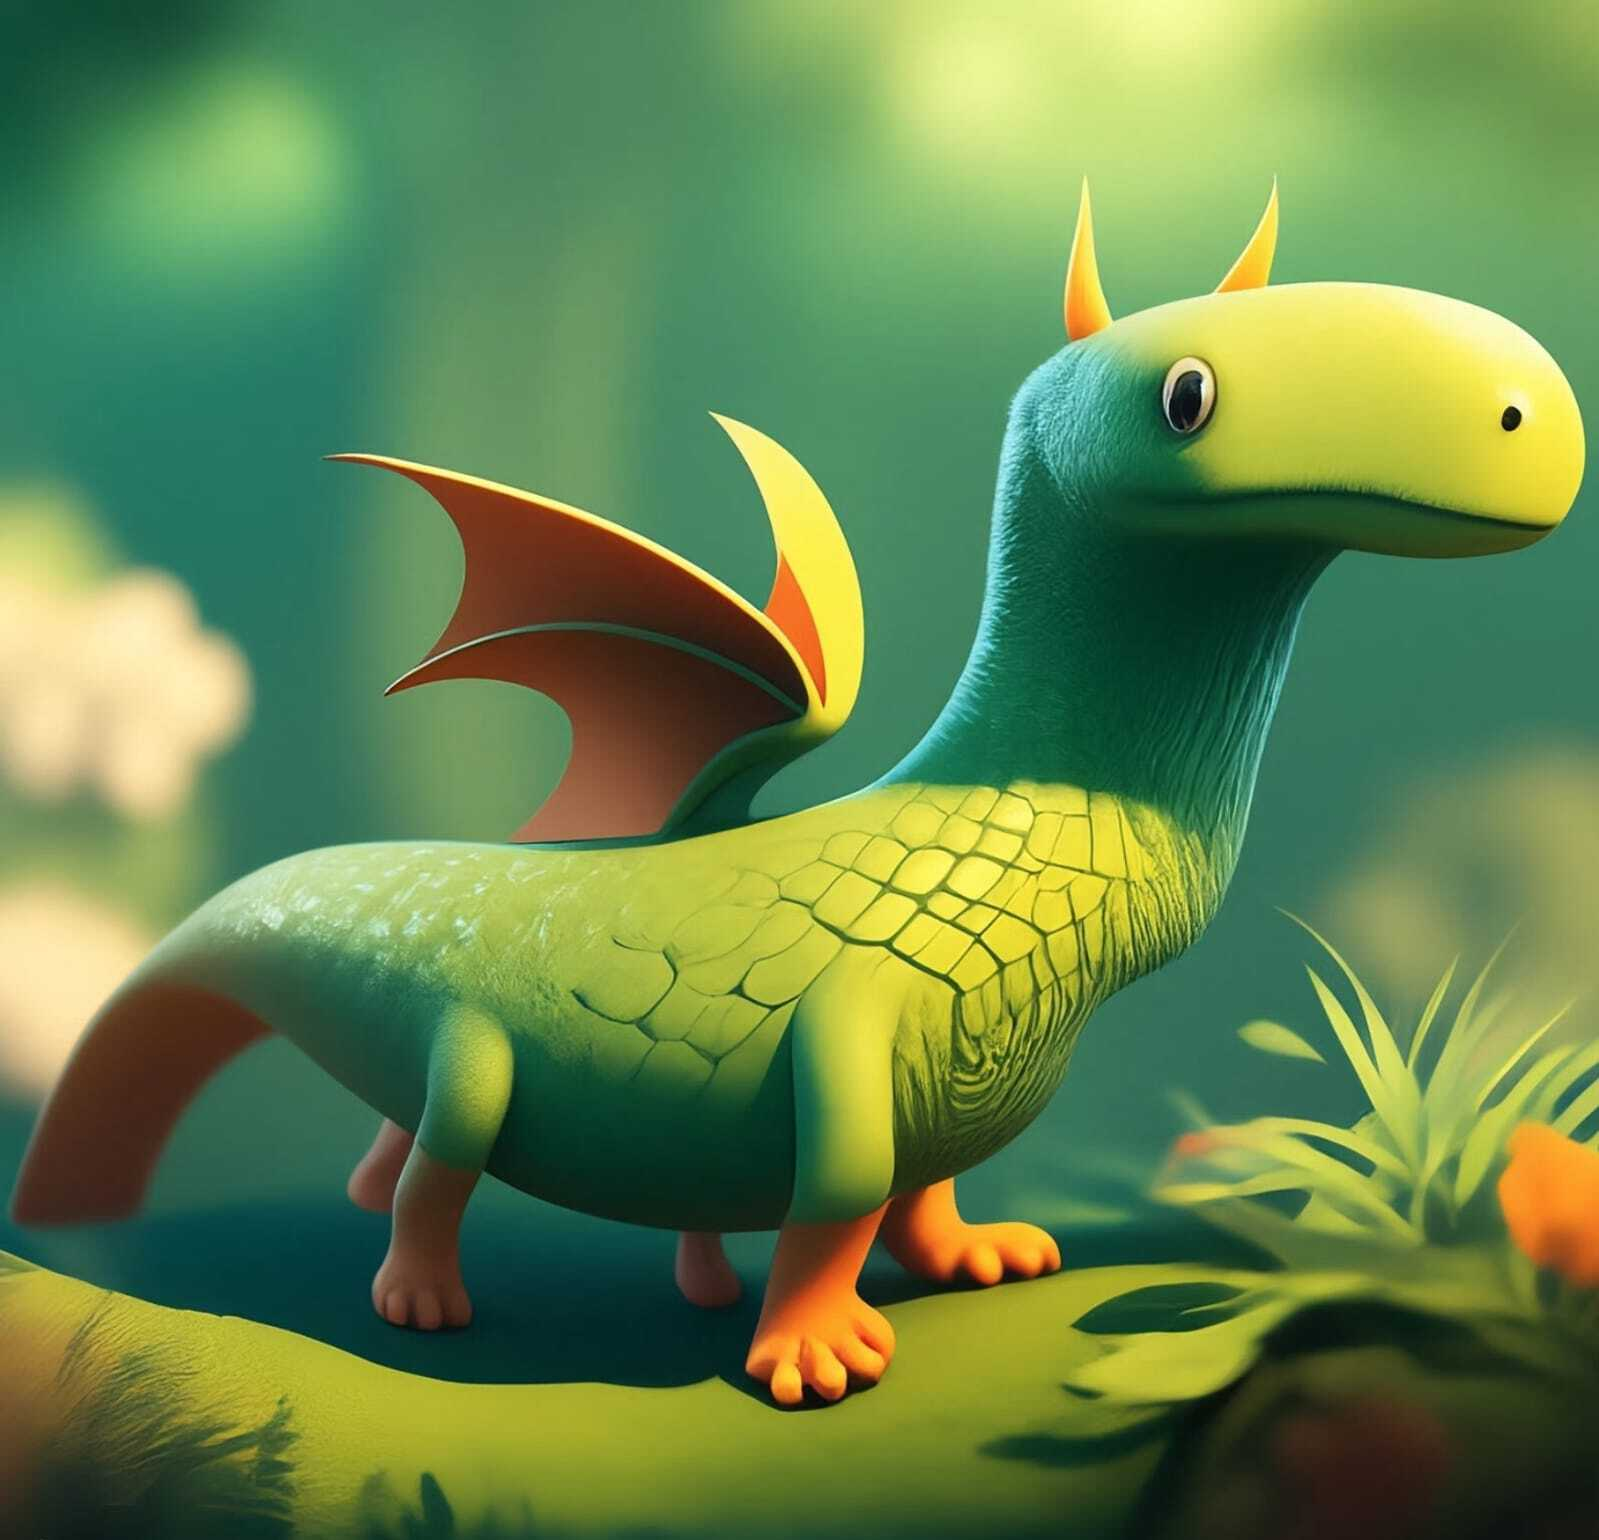
\includegraphics[width=6cm]{cover}
\end{center}
}

% theorem commands
\newtheoremstyle{c_remark}
	{}	% Space above
	{}	% Space below
	{}% Body font
	{}	% Indent amount
	{\bfseries}	% Theorem head font
	{}	% Punctuation after theorem head
	{.5em}	% Space after theorem head
	{\thmname{#1}\thmnumber{ #2}\thmnote{ \normalfont{\text{(#3)}}}}	% head content
\newtheoremstyle{c_definition}
	{3pt}	% Space above
	{3pt}	% Space below
	{}% Body font
	{}	% Indent amount
	{\bfseries}	% Theorem head font
	{}	% Punctuation after theorem head
	{.5em}	% Space after theorem head
	{\thmname{#1}\thmnumber{ #2}\thmnote{ \normalfont{\text{(#3)}}}}	% head content
\newtheoremstyle{c_plain}
	{3pt}	% Space above
	{3pt}	% Space below
	{\itshape}% Body font
	{}	% Indent amount
	{\bfseries}	% Theorem head font
	{}	% Punctuation after theorem head
	{.5em}	% Space after theorem head
	{\thmname{#1}\thmnumber{ #2}\thmnote{ \text{(#3)}}}	% head content

\ifcsname c@english\endcsname
	\theoremstyle{plain}
	\newtheorem{theorem}{Theorem}[section]
	\newtheorem{lemma}[theorem]{Lemma}
	\newtheorem{proposition}[theorem]{Proposition}
	\newtheorem*{proposition*}{Proposition}
	%\newtheorem{corollary}[theorem]{אין חלופה עברית}

	\theoremstyle{definition}
	\newtheorem{definition}[theorem]{Definition}
	\newtheorem*{definition*}{Definition}
	\newtheorem{example}{Example}[section]
	\newtheorem{exercise}{Exercise}[section]

	\theoremstyle{remark}
	\newtheorem*{remark}{Remark}
	\newtheorem*{solution}{Solution}
	\newtheorem{conclusion}[theorem]{Conclusion}
	\newtheorem{notation}[theorem]{Notation}
\else
	\theoremstyle{c_plain}
	\newtheorem{theorem}{משפט}[section]
	\newtheorem{lemma}[theorem]{למה}
	\newtheorem{proposition}[theorem]{טענה}
	\newtheorem*{proposition*}{טענה}
	%\newtheorem{corollary}[theorem]{אין חלופה עברית}

	\theoremstyle{c_definition}
	\newtheorem{definition}[theorem]{הגדרה}
	\newtheorem*{definition*}{הגדרה}
	\newtheorem{example}{דוגמה}[section]
	\newtheorem{exercise}{תרגיל}[section]

	\theoremstyle{c_remark}
	\newtheorem*{remark}{הערה}
	\newtheorem*{solution}{פתרון}
	\newtheorem{conclusion}[theorem]{מסקנה}
	\newtheorem{notation}[theorem]{סימון}
\fi

% Questions related commands
\newcounter{question}
\setcounter{question}{1}
\newcounter{sub_question}
\setcounter{sub_question}{1}

\ifcsname c@english\endcsname
	\newcommand{\question}[1][0]{
		\ifthenelse{#1 = 0}{}{\setcounter{question}{#1}}
		\section{Question \arabic{question}}
		\addtocounter{question}{1}
		\setcounter{sub_question}{1}
	}

	\newcommand{\subquestion}[1][0]{
		\ifthenelse{#1 = 0}{}{\setcounter{sub_question}{#1}}
		\subsection{Part \alph{sub_question}}
		\addtocounter{sub_question}{1}
	}
\else
	\newcommand{\question}[1][0]{
		\ifthenelse{#1 = 0}{}{\setcounter{question}{#1}}
		\section{שאלה \arabic{question}}
		\addtocounter{question}{1}
		\setcounter{sub_question}{1}
	}

	\newcommand{\subquestion}[1][0]{
		\ifthenelse{#1 = 0}{}{\setcounter{sub_question}{#1}}
		\subsection{סעיף \localecounter{letters.gershayim}{sub_question}}
		\addtocounter{sub_question}{1}
	}
\fi

% import lua and start of document
\directlua{common = require ('../common')}

\GetEnv{AUTHOR}

% headers
\author{\AUTHOR}
\date\today

\title{פתרון מטלה 12 --- מבוא ללוגיקה, 80423}

\begin{document}
\maketitle
\maketitleprint{}

\question{}
נשלים את הוכחת עקרון לפשץ.
נסמן ב־$P$ את קבוצת המספרים הראשוניים, ותהי $L = \{ 0, 1, +, \cdot \}$.
נוכיח שהטענות הבאות שקולות עבור פסוק $\varphi$ ב־$L$,
\begin{enumerate}
	\item $\operatorname{ACF}_0 \models \varphi$
	\item $|\{ p \in P \mid \operatorname{ACF}_p \not\models \varphi \}| < \omega$
	\item $|\{ p \in P \mid \operatorname{ACF}_p \models \varphi \}| \ge \omega$
\end{enumerate}
\begin{proof}
	$1 \implies 2$:
	נניח ש־$\operatorname{ACF}_0 \models \varphi$ ולכן משלמות $\operatorname{ACF}_0 \vdash \varphi$, ונוכל להסיק שקיים עץ היסק שמעיד על כך.
	בעץ היסק זה יש שימוש בכמות סופית של טענות, בפרט בכמות סופית של פסוקים $\lnot \varphi_p$ כפי שהוגדרו בתרגול.
	עתה נבחין כי לכל פסוק אחר בעץ ההיסק, הפסוק מוכל ב־$\operatorname{ACF}_p$ לכל $p \in P$ מההגדרה של התורות.
	לכן אם נגדיר $Q \subseteq P$ להיות הקבוצה של הראשוניים כך ש־$\lnot \varphi_n$ בעץ ההיסק, אז לכל $p \in Q$ נוכל להסיק ש־$\operatorname{ACF}_p \lnot\vdash \varphi$.
	אבל מנאותות ושלמות התורות נובע $\operatorname{ACF}_p \not\models \varphi$. לבסוף נבחין שאכן $Q$ סופית ולכן גם קבוצת התורות הללו, זאת מסופיות עץ ההיסק.

	$2 \implies 3$:
	ניזכר ש־$\operatorname{ACF}_p$ שלמה לכל $p \in P$, ונניח ש־$\alpha = |\{ p \in P \mid \operatorname{ACF}_p \not\models \varphi \}| < \omega$. \\*
	לכן נובע ישירות ש־$|\{ p \in P \mid \operatorname{ACF}_p \models \varphi \}| \ge |P| \setminus \alpha = \omega$.

	$3 \implies 1$:
	נגדיר $T_n$ עצי ההיסק המעידים $\operatorname{ACF}_n \models \varphi$ (עם שלמות).
	נעיר שהכוונה היא שעצים אלה מוגדרים עבור המקרים בהם הטענה מתקיימת בהתאם להנחה $\{ p \in P \mid \operatorname{ACF}_p \models \varphi \} \ge \omega$.
	נגדיר בנוסף $A = \{ \varphi_m \mid n < \omega, \varphi_n \in T_n \}$, כלומר קבוצת הפסוקים המעידים על מציין אשר משמשים בהוכחת $\varphi$ באיזשהו עץ ההיסק.
	נניח שהיא לא ריקה ולכן יהי $\varphi_n \in A$, אז נוכל להסיק ש־$T \vdash (\varphi_n \to \varphi)$, כאשר $T$ תורת השדות הסגורים אלגברית.
	אבל $\operatorname{ACF}_m \models \lnot \varphi_n$ לכל $m \ne n$ וזו סתירה להנחה, לכן $\varphi_n \notin A$.
	אז $|A| = 0$, נבחר $T_n$ כלשהו ולכן $\lnot \varphi_m \in T_n$ לאיזושהי קבוצת ערכים $m < \omega$, ובהתאם עץ היסק זה תקין גם ב־$\operatorname{ACF}_0$, ולכן מנאותות נובע $\operatorname{ACF}_0 \models \varphi$.
\end{proof}

\question{}
נבחין בהגדרת $r: \operatorname{form}_L \to \NN$ אשר הופיעה בהרצאה.
תהי $\varphi$ נוסחה.

\subquestion{}
נוכיח ש־$r(\varphi)$ הוא גובה עץ היצירה של $\varphi$ לכל $\varphi \in \operatorname{form}_L$.
\begin{proof}
	נגדיר $B = \{ x \in 2^n \mid n < \omega\}$, קבוצת כל הענפים האפשריים בעצים סטנדרטיים מיושרים לשמאל.
	נגדיר גם $b_m : \operatorname{form}_L \to B$ כך ש־$b_m(\varphi) = \sup \{ b \in B \mid b \in \varphi \}$, כאשר $b \in \varphi$ אם ורק אם קיים הענף $b$ בעץ היצירה של $\varphi$, ביחס הסדר של עץ יצירה זה.
	אנו רוצים להוכיח ש־$|b_m(\varphi)| = r(\varphi)$ לכל $\varphi \in \operatorname{form}_L$.

	נוכיח את הטענה באינדוקציה על מבנה הנוסחה.
	לבסיס נניח ש־$\varphi$ נוסחה יסודית, ולכן $r(\varphi) = 1$ לפי הגדרת הפונקציה, בעוד $b_m(\varphi) = \langle \rangle$ לפי הגדרת $b_m$, ולכן נובע $|b_m(\varphi)| = 1 = r(\varphi)$.
	נניח שהטענה נכונה עבור $\varphi$ ונבחן את $\lnot \varphi$, מהגדרת $r$, $r(\lnot \varphi) = r(\varphi) + 1 = |b_m(\varphi)| + 1$.
	מהצד השני $b_m(\lnot \varphi) = \langle 0 \rangle \frown b_m(\varphi)$, ולכן $|b_m(\lnot \varphi)| = 1 + |b_m(\varphi)| = r(\lnot \varphi)$.
	נניח ש־$\psi$ מקיים אף הוא את הטענה ויהי $\square \in \Bb$, ונבחן את $\varphi \square \psi$.
	נובע $r(\varphi \square \psi) = \max\{r(\varphi), r(\psi)\} + 1$ מהגדרה, וכן $b_m(\varphi \square \psi) = \sup\{ \langle 0 \rangle \frown b_m(\varphi), \langle 1 \rangle \frown b_m(\psi)\}$.
	לכן $|b_m(\varphi \square \psi)| = 1 + \max\{|b_m(\varphi)|, |b_m(\psi)|\} = r(\varphi \square \psi)$.
	נבחן עתה את $\forall v \varphi$, במקרה זה מוגדר $r(\forall v \varphi) = r(\varphi) + 1$ וכן $b_m(\forall v \varphi) = \langle 0 \rangle \frown b_m(\varphi)$,
	ולכן $|b_m(\forall v \varphi)| = 1 + |b_m(\varphi)| = r(\forall v \varphi)$.
	סיימנו את מהלך האינדוקציה.
\end{proof}

\subquestion{}
נוכיח שמתקיים $r(\varphi) = r(\varphi_t^x)$ לכל $t \in \operatorname{constterm}_L$ ולכל $x \in \operatorname{Var}$.
\begin{proof}
	מהגדרת החלפה ועץ היצירה נבחין שאם $\langle T, f \rangle$ עץ היצירה של $\varphi$ אז $f(b_m(\varphi) \restriction 2^n) = f(b_m(\varphi_t^x) \restriction 2^n)$ לכל $n < |b_m(\varphi)|$.
	נבחין גם שמתקיים ${f(b_m(\varphi))}_t^x = f(b_m(\varphi_t^x))$ ולכן $r(\varphi) = r(\varphi_t^x)$.
\end{proof}

\question{}
תהי $L = \{ E \}$ שפה עם סימן יחס דו־מקומי.

\subquestion{}
נכתוב אקסיומות לתורה $T$ כך ש־$E$ יהיה יחס שקילות שכל מחלקותיו באותו הגודל.
\begin{solution}
	\begin{align*}
		& T = \{ \forall x (E(x, x)), \forall x \forall y (E(x, y) \to E(y, x)), \forall x \forall y \forall z ((E(x, y) \land E(y, z)) \to E(x, z)) \} \\
		& \cup \{ \forall x_0, \dots, x_n, y_0, \dots, y_{n - 1} (\forall i < j < n (x_i \ne x_j \land y_i \ne y_j \land E(x_i, x_j) \land E(y_i, y_j)) \land E(x_0, x_n) \land \forall i < n, x_n \ne x_i) \\
		& \to \exists y_n (E(y_0, y_n) \land \forall i < n, y_n \ne y_i) \mid n < \omega \}
	\end{align*}
	כלומר לכל קבוצות איברים ממחלקות שקילות שונות מגודל סופי, אם נוסיף איבר לקבוצה של מחלקת השקילות הראשונה, נוכל להוסיף גם איבר לקבוצה של מחלקת השקילות השנייה.
	דהינו לכל מספר סופי, קבוצות ממחלקות השקילות הן בנות הרחבה לאותו גודל.
	בשל כך גם למקרים בני־מניה נוכל לקבל שהמחלקות הן באותו גודל, אבל לא עבור מקרים גדולים יותר.
\end{solution}

\subquestion{}
נגדיר קבוצה $\operatorname{comp}(T)$ של תורות שלמות המכילות את $T$.
נראה שכל תורה שלמה $T_0 \supseteq T$ שקולה לתורה $T_0' \in \operatorname{comp}(T)$, במובן שמתקיים $\forall \varphi, T_0 \models \varphi \iff T_0' \models \varphi$.
\begin{solution}
	אנו יודעים ש־$|\operatorname{sent}_L| = \omega$ ולכן נגדיר $\operatorname{comp}(T) = \{ S \subseteq \operatorname{sent}_L \mid S \text{ is complete}, T \subseteq S \}$.
	זוהי קבוצה ומתקיים $|\operatorname{comp}(T)| \le \omega_1$.
	מההגדרה נובע שאם $T_0 \supseteq T$ תורת שלמה, אז $T_0 \in \operatorname{comp}(T)$ ולכן בפרט נובע $\forall \varphi, T_0 \models \varphi \iff T_0 \models \varphi$ כפי שרצינו.

	נעיר שמותר לנו להשתמש באקסיומת הפרדה כפי שעשינו שכן נוכל להשתמש בפונקציית הערכת האמת כל קבוצת כל המודלים $\le \omega$ כדי להגדיר פונקציה בוליאנית שמחזירה עבור כל תורה האם יש בה סתירה.
\end{solution}

\subquestion{}
נבדוק אילו מהתורות ב־$\operatorname{comp}(T)$ הן $\aleph_0$־קטגוריות ואילו קטגוריות.
\begin{solution}
	כל תורה שקובעת ביחידות את גודל ומספר מחלקות השקילות שלה תקבע באופן יחיד את המודלים שלה, שכן נוכל לבנות איזומורפיזם של תורת הקבוצות בין כל שני מודלים ביחס לקבוצות של מחלקות השקילות.
	כל תורה שלא מאפשרת כמות סופית של מחלקות שקילות או של גודלן, תהיה $\aleph_0$־קטגורית מסיבות דומות.
\end{solution}

\question{}
נפריך את הטענה שכל תורה $\aleph_0$־קטגורית היא שלמה.
\begin{solution}
	נעבוד בשפת השוויון, כלומר $L = \{ = \}$.
	נקבע $c < \omega$ כלשהו, ונגדיר את $T_c = \{ \varphi_{\ge n} \mid n < c \}$.

	נוכיח ש־$T_c$ היא $\aleph_0$־קטגורית.
	יהיו מודלים $\Aa, \Bb \models T_c$ כך ש־$|A| = |B| = \aleph_0$.
	משוויון העוצמות נובע שקיימת $f : A \to B$ חד־חד ערכית ועל.
	נובע אם כך ש־$\forall a, a', a = a' \iff f(a) = f(a')$, אבל מהגדרת השוויון גם $a =^\Aa a' \iff f(a) =^\Bb f(a')$, לכן $f : \Aa \to \Bb$ איזומורפיזם ובהתאם $T_c$ היא $\aleph_0$־קטגורית.

	אבל נבחין ש־$\langle [c + 1], = \rangle \models T_c, \varphi_{\ge c + 1}$, וכן ש־$\langle [c], = \rangle \models T_C, \lnot \varphi_{\ge n + 1}$, לכן $T_c$ היא לא שלמה, בסתירה לטענה.
\end{solution}

\question{}
תהי $L$ שפה לתחשיב יחסים.
יהי $x$ משתנה ונניח ש־$\varphi$ פסוק.
תהי $\Sigma$ קבוצת פסוקים כך ש־$\Sigma \models \varphi_c^x$ עבור קבוע $c$ שאינו מופיע ב־$\varphi$ או ב־$\Sigma$.

\subquestion{}
נוכיח ללא שימוש במשפטי השלמות והנאותות ש־$\Sigma \models \forall \varphi$.
\begin{proof}
	נבחין שמתקיים $\Sigma \models \varphi_c^x$ אם ורק אם לכל $\Mm \in \operatorname{Mod}(\Sigma)$ מתקיים $\Mm \models \varphi_c^x$.
	נבחין שאם נבחר מודל $\Mm$ כזה, אז $c^\Mm = d$ עבור איזשהו $d \in M$.
	אבל עבור מודל $\Nn$ כך ש־$N = M$ ופירוש כל סימן ב־$\Nn$ זהה לזה ב־$\Mm$ פרט ל־$c^\Nn = x$ כלשהו, עדיין מתקיים $\Nn \models \varphi_c^x$,
	ולכן נוכל להסיק $\Mm \models \varphi_d^x$ לכל $d \in M$, כלומר $\Mm \models \forall x \varphi$.
	טענה זו נכונה עבור כל מודל $\Mm$ כזה, לכן בפרט מההגדרה $\Sigma \models \forall x \varphi$.
\end{proof}

\subquestion{}
נראה שלא בהכרח $\varphi_c^x \models \forall x \varphi$.
\begin{solution}
	נגדיר את השפה $L = \{ =, c \}$ וכן את המודל $\Mm = \langle 2; 0 \rangle$, וכן $\varphi = x = c$.
	לכן מתקיים $\varphi_c^x$, כלומר $\Mm\ models 0 = 0$, אבל $\Mm \models \forall x \varphi \implies \Mm \models \varphi_1^x$, כלומר $\Mm \models 1 = 0$, וזו כמובן סתירה.
\end{solution}

\end{document}
